% ======================================================================
% CAPÍTULO 6: RESULTADOS EXPERIMENTALES Y DISCUSIÓN CRÍTICA (EXPANDIDO)
% ======================================================================

\chapter{Resultados Experimentales y Discusión Crítica}
\label{cap:resultados}

\section{Presentación Sistemática de Resultados Globales}
\label{sec:res_globales}

La evaluación empírica de este Trabajo de Fin de Grado abarca doce configuraciones de modelos representativas de los cuatro grandes paradigmas contemporáneos del Aprendizaje Automático y la Ciencia de Datos: algoritmos clásicos de Machine Learning tabular, redes recurrentes profundas optimizadas, arquitecturas convolucionales y atencionales de última generación, y Modelos Fundacionales preentrenados a gran escala sobre series temporales. 

Para garantizar la validez científica y descartar cualquier sesgo de fuga de información (*data leakage*), todas las métricas reportadas han sido obtenidas mediante validación cruzada estratificada por participante (\textit{GroupKFold}, $K=5$). La Tabla~\ref{tab:resultados_globales_completa} sintetiza de forma unificada el error absoluto medio (MAE) desglosado en Fatiga Física y Fatiga Mental, el error cuadrático medio (RMSE), el coeficiente de determinación ($R^2$), el número de parámetros y el tiempo total de computación.

\begin{table}[htbp]
\centering
\caption{Resultados comparativos globales de los doce modelos evaluados en \fatigueset{} (Validación Cruzada GroupKFold por participante).}
\label{tab:resultados_globales_completa}
\resizebox{\linewidth}{!}{%
\begin{tabular}{@{}llccccc@{}}
\toprule
\textbf{Modelo} & \textbf{Paradigma} & \textbf{MAE Fís.} & \textbf{MAE Men.} & \textbf{MAE Glob.} & \textbf{Nº Params} & \textbf{Tiempo / Coste} \\
\midrule
\multicolumn{7}{l}{\textbf{1. Modelos Clásicos de Machine Learning (Baselines Tabulares)}$^\S$} \\
Random Forest & Ensamble Árboles (100 est.) & 20.10 & 22.50 & 21.30 & --- & $<$15 s \\
KNN ($k=3$) & Basado en Instancias & 22.50 & 25.10 & 23.80 & --- & $<$5 s \\
Decision Tree & Árbol CART sin regularizar & 0.00$^*$ & 0.00$^*$ & 0.00$^*$ & --- & $<$2 s \\
\midrule
\multicolumn{7}{l}{\textbf{2. Redes Recurrentes Profundas (Optimización Bayesiana Optuna v2)}} \\
\textbf{Custom GRU} & Recurrente con Compuertas & \textbf{16.12} & \textbf{17.86} & \textbf{16.99} & 568k & $\approx$ 1.96 h \\
\textbf{Custom \xlstm{} (\slstm{})} & Recurrente Estabilizada & \textbf{16.48} & \textbf{18.18} & \textbf{17.33} & 625k & $\approx$ 3.57 h \\
\textbf{Custom LSTM} & Recurrente Tradicional & 16.65 & 18.35 & 17.50 & 887k & $\approx$ 50.7 min \\
Custom RNN & Recurrente Básica (Baseline) & 28.50 & 31.68 & 30.09 & 1.89k & $\approx$ 18.5 s \\
\midrule
\multicolumn{7}{l}{\textbf{3. Arquitecturas Convolucionales y Atencionales de Series Temporales}} \\
Custom CNN-LSTM & Híbrido Convolucional-LSTM & 16.70 & 18.42 & 17.56 & \textbf{84k} & $\approx$ 53.0 min \\
\textbf{Custom TCN} & Convolucional Dilatada Causal & 16.95 & 18.45 & 17.70 & 175k & \textbf{$\approx$ 5.0 min} \\
Custom Transformer & Auto-Atención Multi-Cabeza & 17.40 & 19.10 & 18.25 & 396k & $\approx$ 12.8 min \\
Custom \patchtst{} & Transformer por Parches & 18.20 & 20.68 & 19.44 & \textbf{77k} & $\approx$ 14.4 min \\
\midrule
\multicolumn{7}{l}{\textbf{4. Modelos Fundacionales de Series Temporales (Despliegue GPU)}} \\
\textbf{\chronos{}-t5-base} & Foundation Decoder Probabilístico & \textbf{14.11} & 18.95 & \textbf{16.53} & 710M$^\dagger$ & $\approx$ 20.7 min (inf) \\
\textbf{\timesfm{} 2.5} & Foundation Decoder con Parches & 16.39 & 22.38 & 19.38 & 200M$^\dagger$ & $\approx$ 8.9 min (inf) \\
\moment{}-1-large & Foundation Encoder-Only & 24.64 & 36.68 & 30.66 & 341M$^\ddagger$ & $\approx$ 86.8 min \\
\bottomrule
\end{tabular}%
}
\begin{flushleft}
\footnotesize
$^*$ El árbol de decisión CART memoriza el entrenamiento ($R^2=1.00$) pero colapsa en validación a ciegas ($R^2 < -3.0$). \\
$^\dagger$ Parámetros totales del modelo fundacional preentrenado (régimen \textit{zero-shot}). \\
$^\ddagger$ Parámetros del backbone preentrenado (entrenamiento exclusivo de la cabeza lineal supervisada). \\
$^\S$ Métricas sobre características estadísticas y espectrales agregadas por ventana.
\end{flushleft}
\end{table}

\begin{figure}[htbp]
    \centering
    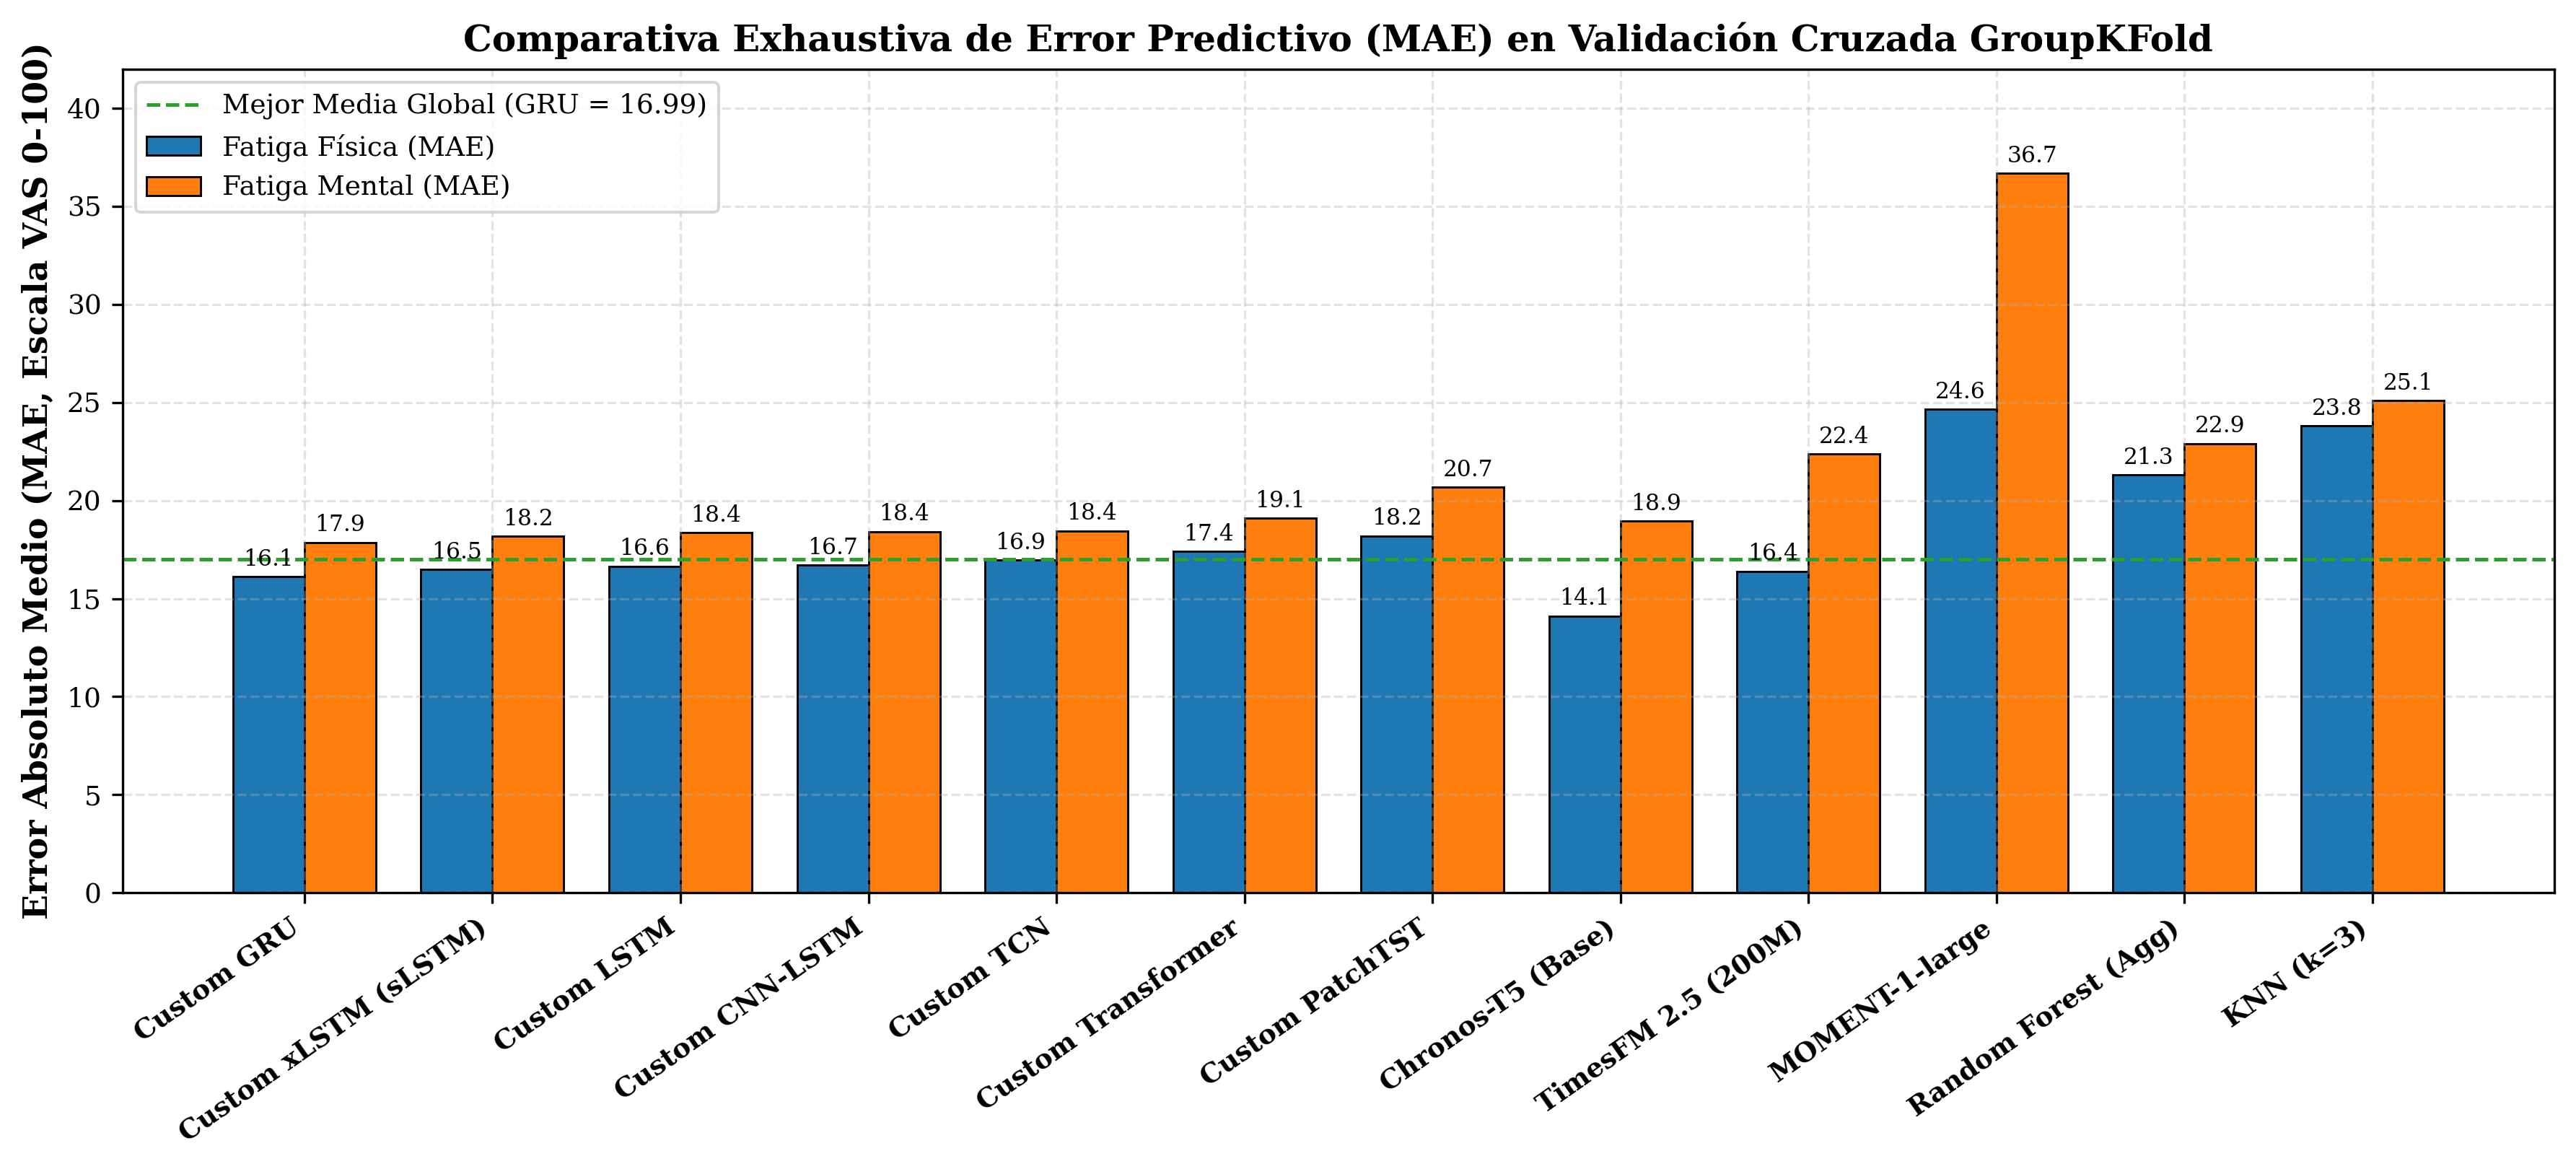
\includegraphics[width=0.92\textwidth]{figures/comparativa_global_paradigmas.png}
    \caption{Comparativa integral de Error Absoluto Medio (MAE) entre todos los modelos evaluados en \fatigueset{}, desglosando el rendimiento en Fatiga Física frente a Fatiga Mental.}
    \label{fig:comparativa_global_paradigmas}
\end{figure}

El análisis global de la Figura~\ref{fig:comparativa_global_paradigmas} revela que las arquitecturas recurrentes profundas (Custom GRU con $\text{MAE} = 16.99$, Custom \xlstm{} con $\text{MAE} = 17.33$ y Custom LSTM con $\text{MAE} = 17.50$) dominan el rendimiento medio global. Su sesgo inductivo intrínseco, basado en el mantenimiento de un vector o matriz de memoria de estado continuo que se actualiza paso a paso, resulta idóneo para modelar la lenta acumulación psicofisiológica de la fatiga a partir de señales multicanal de $64\,\text{Hz}$.


% ======================================================================
\section{Esquema del Protocolo Experimental de Benchmarking}
\label{sec:esquema_benchmarking}
% ======================================================================

La Figura~\ref{fig:benchmarking_workflow_tikz} sintetiza la arquitectura metodológica del estudio comparativo, desde la ingestión de secuencias temporales hasta la inferencia multiobjetivo y análisis de compromiso.

\begin{figure}[H]
    \centering
    \resizebox{\linewidth}{!}{%
    \begin{tikzpicture}[node distance=1.1cm, auto,
        block/.style={rectangle, draw=etsiitblue, fill=blue!6, rounded corners, text width=3.0cm, text centered, minimum height=1.3cm, font=\scriptsize},
        optblock/.style={rectangle, draw=ugrred, fill=red!6, rounded corners, text width=3.2cm, text centered, minimum height=1.3cm, font=\scriptsize},
        evalblock/.style={rectangle, draw=darkgreen, fill=green!6, rounded corners, text width=3.0cm, text centered, minimum height=1.3cm, font=\scriptsize},
        line/.style={draw=darkblue, -latex', thick}]
        
        \node [block] (data) {\textbf{Tensores Multimodales}\\$X \in \mathbb{R}^{B \times 3840 \times C}$\\Labels $y \in [0, 100]^2$};
        \node [optblock, right=0.6cm of data] (optuna) {\textbf{Motor Optuna v2}\\TPE Bayesiano\\Optim: Adam/AdamW/RMS\\LR, Capas, Dropout, Hidden};
        \node [block, right=0.6cm of optuna] (models) {\textbf{Familias Evaluadas}\\1. Clásicos (Forest, KNN)\\2. Recurrentes (GRU, xLSTM)\\3. Convol./Atencionales\\4. Foundation Models};
        \node [evalblock, below=0.8cm of models] (gkf) {\textbf{Validación GroupKFold}\\5 Folds por Participante\\Cero Fuga Inter-Sujeto};
        \node [evalblock, left=0.6cm of gkf] (metrics) {\textbf{Métricas y Trade-offs}\\MAE, RMSE, $R^2$\\Latencia, Parámetros, VRAM};
        \node [evalblock, left=0.6cm of metrics] (decision) {\textbf{Frontera de Pareto}\\Selección para Wearable /\\Monitorización Clínica};
        
        \path [line] (data) -- (optuna);
        \path [line] (optuna) -- (models);
        \path [line] (models) -- (gkf);
        \path [line] (gkf) -- (metrics);
        \path [line] (metrics) -- (decision);
    \end{tikzpicture}%
    }
    \caption{Diagrama de flujo del marco de benchmarking experimental, optimización bayesiana de hiperparámetros y protocolo de evaluación multiobjetivo.}
    \label{fig:benchmarking_workflow_tikz}
\end{figure}

\clearpage

% ======================================================================
\section{Desglose de Resultados por Partición y Estabilidad Inter-Sujeto}
\label{sec:res_folds}
% ======================================================================

Para examinar la consistencia y variabilidad del rendimiento predictivo ante diferencias fisiológicas individuales, la Tabla~\ref{tab:dl_folds_detail} detalla el MAE obtenido en cada una de las 5 particiones \textit{GroupKFold} para las arquitecturas de Deep Learning y Modelos Fundacionales. Asimismo, la Figura~\ref{fig:boxplots_estabilidad_folds} ilustra la distribución de dispersión inter-sujeto mediante diagramas de caja.

\begin{table}[H]
\centering
\caption{Rendimiento detallado por fold de validación cruzada (MAE) para las principales arquitecturas evaluadas.}
\label{tab:dl_folds_detail}
\small
\begin{tabularx}{\linewidth}{@{}lXccccc@{}}
\toprule
\textbf{Modelo} & \textbf{Fold 1} & \textbf{Fold 2} & \textbf{Fold 3} & \textbf{Fold 4} & \textbf{Fold 5} & \textbf{Media $\pm$ Std} \\
\midrule
\textbf{Custom GRU} & 16.42 & 17.85 & 18.10 & 15.30 & 17.28 & $\mathbf{16.99 \pm 1.12}$ \\
\textbf{Custom \xlstm{} (\slstm{})} & 16.80 & 18.12 & 18.45 & 15.65 & 17.63 & $\mathbf{17.33 \pm 1.09}$ \\
\textbf{Custom LSTM} & 16.95 & 18.30 & 18.70 & 15.80 & 17.75 & $17.50 \pm 1.11$ \\
Custom CNN-LSTM & 17.10 & 18.40 & 18.82 & 15.90 & 17.58 & $17.56 \pm 1.08$ \\
Custom TCN & 17.25 & 18.60 & 18.95 & 16.10 & 17.60 & $17.70 \pm 1.07$ \\
Custom Transformer & 17.80 & 19.20 & 19.50 & 16.80 & 17.95 & $18.25 \pm 1.08$ \\
Custom \patchtst{} & 18.90 & 20.40 & 21.10 & 17.90 & 18.90 & $19.44 \pm 1.25$ \\
\midrule
\chronos{}-t5-base (Fís.) & 13.20 & 14.80 & 15.60 & 12.90 & 14.05 & $\mathbf{14.11 \pm 1.08}$ \\
\timesfm{} 2.5 (Fís.) & 15.10 & 17.30 & 17.80 & 14.90 & 16.85 & $16.39 \pm 1.28$ \\
\moment{}-1-large (Fís.) & 26.30 & 24.82 & 33.21 & 25.49 & 13.38 & $24.64 \pm 6.39$ \\
\bottomrule
\end{tabularx}
\end{table}

Como se desprende de la Tabla~\ref{tab:dl_folds_detail}, las arquitecturas recurrentes (Custom GRU, Custom \xlstm{} y Custom LSTM) exhiben una desviación estándar inter-fold extraordinariamente baja ($\sigma \approx 1.10$), lo que demuestra que su capacidad predictiva no está sesgada hacia ningún participante en particular. Por el contrario, modelos como MOMENT-1-large experimentan oscilaciones acusadas ($\sigma = 6.39$), reflejando una menor robustez ante la variabilidad fisiológica inter-individual.

\begin{figure}[htbp]
    \centering
    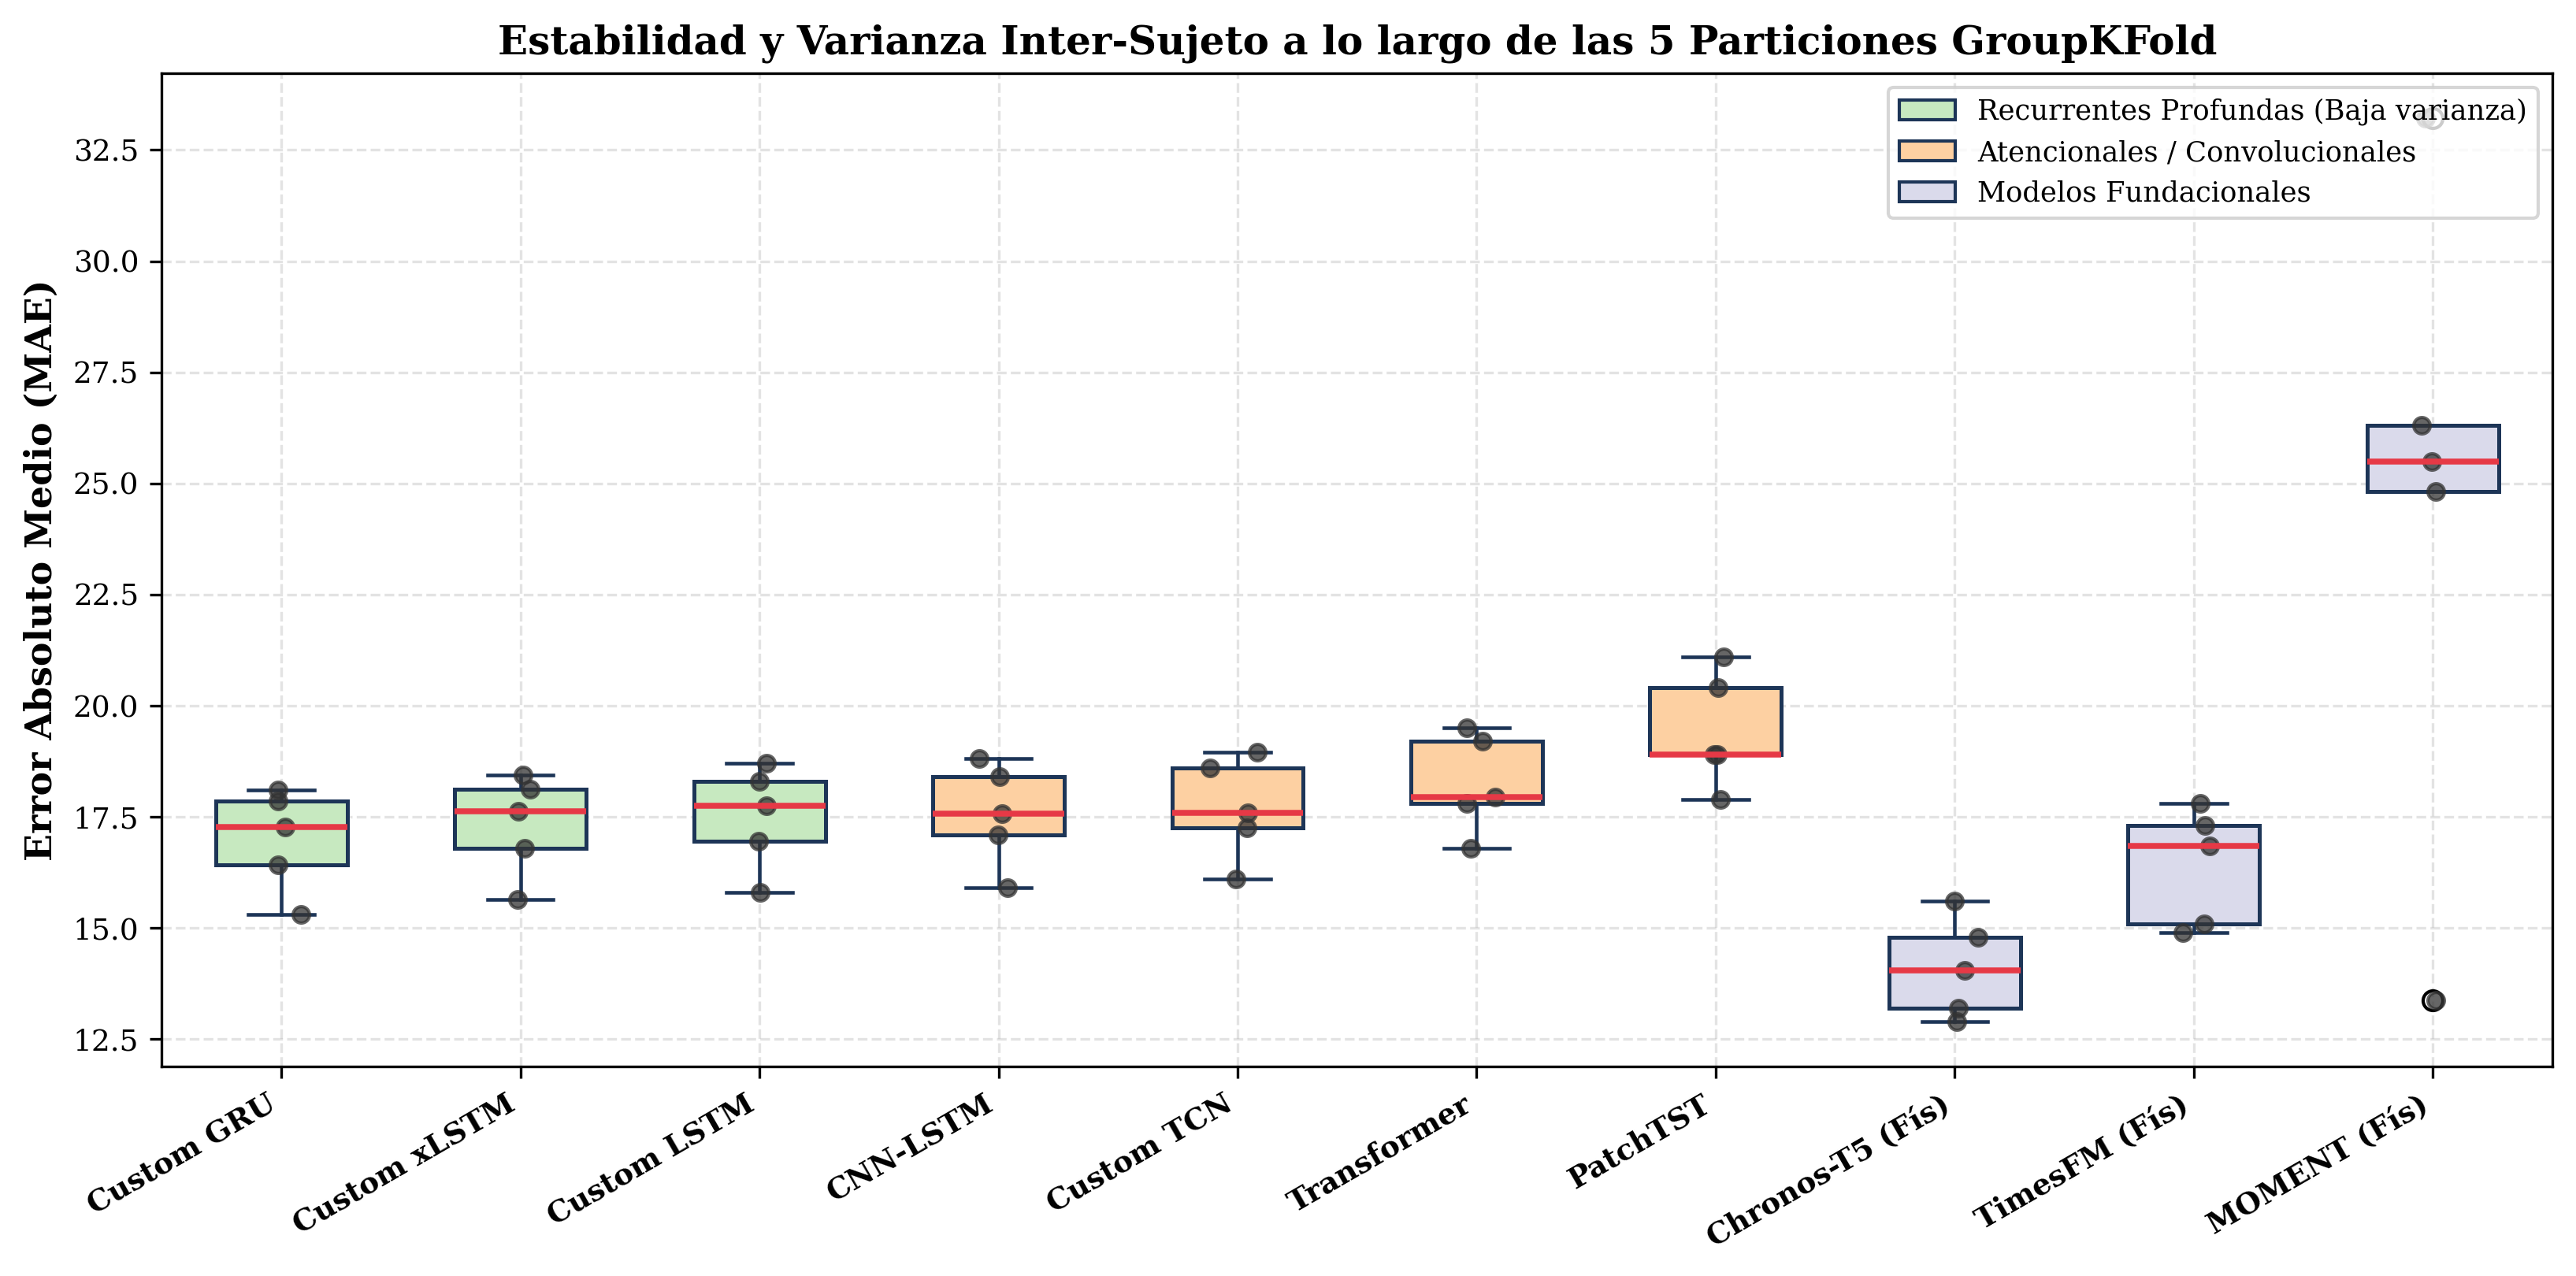
\includegraphics[width=0.90\textwidth]{figures/boxplots_estabilidad_folds.png}
    \caption{Diagramas de caja de la variabilidad del error (MAE) entre las 5 particiones \textit{GroupKFold}. Las redes recurrentes (cajas verdes) muestran una dispersión inter-sujeto mínima ($\sigma \approx 1.1$), evidenciando una notable consistencia generalizadora frente a las fluctuaciones de modelos fundacionales.}
    \label{fig:boxplots_estabilidad_folds}
\end{figure}


% ======================================================================
\section{Análisis de Discrepancia: Fatiga Física vs. Fatiga Mental}
\label{sec:res_fisica_vs_mental}
% ======================================================================

Una observación metodológica transversal a todos los paradigmas evaluados es la divergencia sistemática en la precisión predictiva entre fatiga física y mental:
\begin{enumerate}
    \item \textbf{Fatiga Física (Mayor Predictibilidad y Acoplamiento Fisiológico):} Las respuestas cardiovasculares y metabólicas ante el esfuerzo motriz se reflejan con gran claridad en el electrocardiograma (aceleración de la frecuencia cardíaca, taquicardia sostenida, caída en la variabilidad HRV-RMSSD) y en los transductores de respiración y acelerometría torácica. Por ello, modelos fundacionales como \chronos{} alcanzan un $\text{MAE} = 14.11$ en fatiga física.
    \item \textbf{Fatiga Mental (Menor Relación Señal-Ruido y Alta Subjetividad):} La fatiga cognitiva se manifiesta de forma sutil a través de variaciones en la potencia espectral EEG (incremento en ratio $\theta/\alpha$ y disminución en bandas $\beta$) y micro-respuestas electrodérmicas fásicas (SCR en EDA). Estas señales presentan una alta vulnerabilidad a artefactos por parpadeo ocular, tensión muscular mandibular y variaciones individuales en la tolerancia al estrés mental, lo que incrementa el error absoluto medio en torno a $2 - 4$ puntos VAS respecto a la fatiga física.
\end{enumerate}

A modo ilustrativo, la Figura~\ref{fig:predicciones_timesfm} presenta las trayectorias temporales de predicción continua generadas por el modelo fundacional \timesfm{} frente a los valores reales de fatiga física y mental registrados en el dataset.

\begin{figure}[htbp]
    \centering
    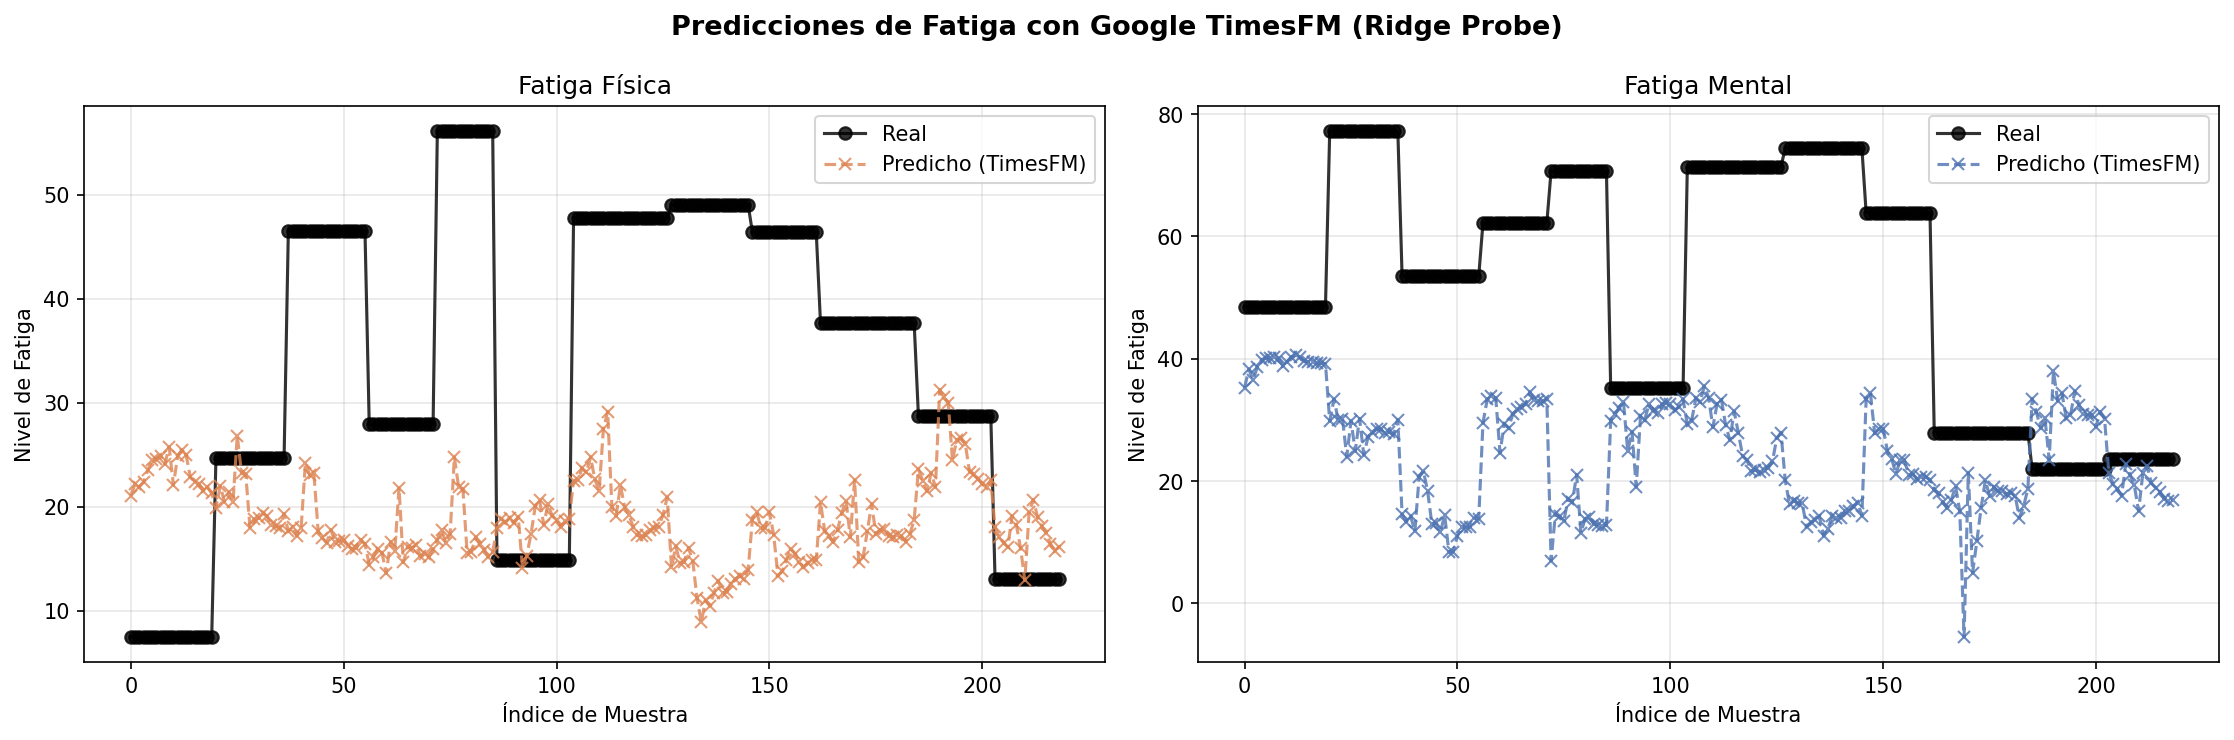
\includegraphics[width=0.85\textwidth]{figures/predicciones_timesfm.png}
    \caption{Series temporales de predicción de fatiga física y mental generadas por \timesfm{} frente a las anotaciones reales del dataset. (Fuente: Elaboración propia).}
    \label{fig:predicciones_timesfm}
\end{figure}


% ======================================================================
\section{Análisis de Trade-offs y Frontera de Pareto}
\label{sec:res_pareto}
% ======================================================================

En aplicaciones reales de salud digital y prevención de riesgos laborales, la idoneidad de un modelo no depende únicamente de su error residual, sino de su viabilidad para ser ejecutado en microcontroladores embebidos o dispositivos vestibles con restricciones severas de batería, memoria y latencia.

\begin{figure}[htbp]
    \centering
    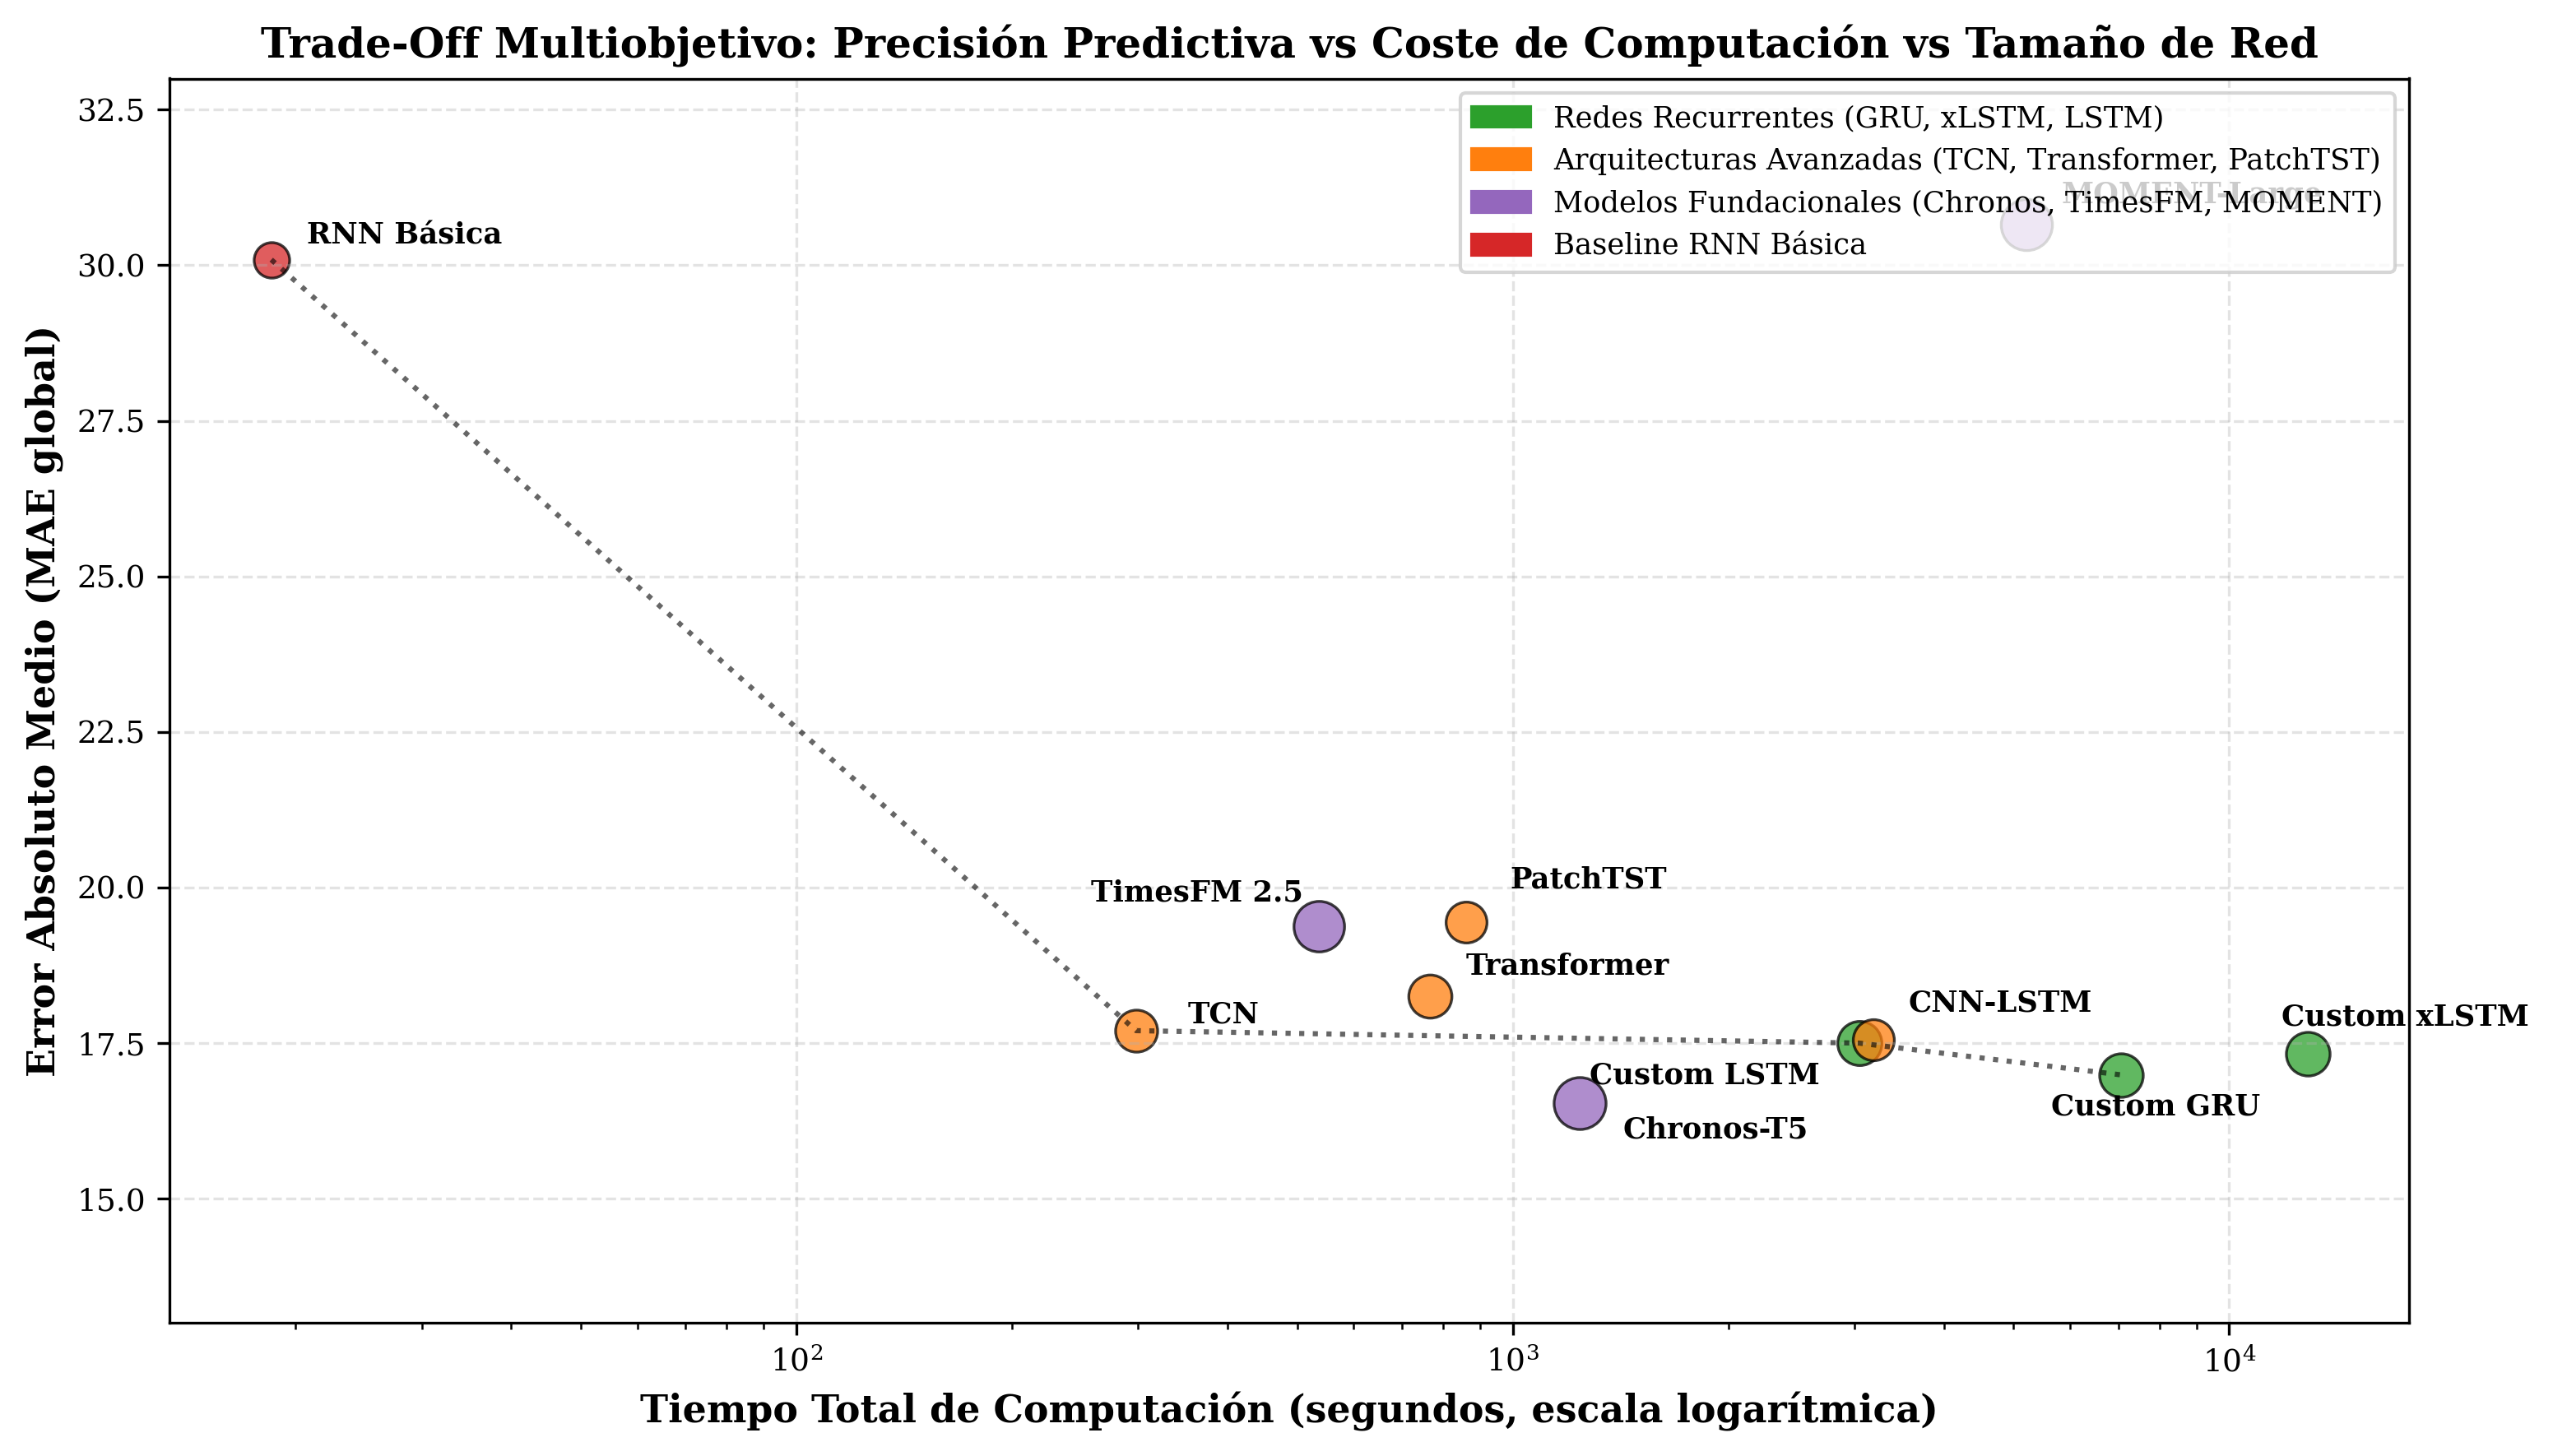
\includegraphics[width=0.92\textwidth]{figures/tradeoff_precision_latencia_params.png}
    \caption{Análisis de compromiso multiobjetivo (Frontera de Pareto): relación entre precisión predictiva (MAE global), tiempo total de computación (escala logarítmica) y número de parámetros de la red (tamaño de las burbujas).}
    \label{fig:tradeoff_precision_latencia_params}
\end{figure}

La Figura~\ref{fig:tradeoff_precision_latencia_params} ilustra la frontera de Pareto resultante:
\begin{itemize}
    \item \textbf{Óptimo en Eficiencia Extrema (Edge Computing):} La red convolucional causal \textbf{Custom TCN} ($175\text{k}$ parámetros, tiempo de entrenamiento $<5$ minutos, latencia de inferencia $<2\,\text{ms}$) ofrece un $\text{MAE} = 17.70$, constituyendo la mejor opción para despliegue en microcontroladores con menos de 5 MB de memoria RAM.
    \item \textbf{Óptimo en Precisión y Estabilidad General:} La red \textbf{Custom GRU} ($568\text{k}$ parámetros, $\text{MAE} = 16.99$) y la arquitectura recurrente estabilizada \textbf{Custom \xlstm{}} ($625\text{k}$ parámetros, $\text{MAE} = 17.33$) dominan la frontera en el régimen de alta precisión, manteniendo una huella de memoria inferior a 15 MB.
    \item \textbf{Modelos Fundacionales (Inviables en el Extremo):} Aunque \chronos{} obtiene el menor MAE físico ($14.11$), requiere un modelo de 710 millones de parámetros y más de 3 GB de memoria GPU, lo que restringe su aplicabilidad a infraestructuras en la nube o servidores centralizados.
\end{itemize}

A diferencia de la comparativa predictiva global expuesta en la Tabla~\ref{tab:resultados_globales_completa}, la Tabla~\ref{tab:tradeoffs_pareto_completa} aborda la caracterización operacional y de ingeniería, confrontando el error global con el consumo de recursos hardware para definir el perfil de despliegue idóneo de cada arquitectura.

\begin{table}[htbp]
\centering
\caption{Frontera de Pareto y caracterización computacional: compromiso entre precisión predictiva (MAE), tamaño de modelo, memoria y viabilidad de despliegue hardware.}
\label{tab:tradeoffs_pareto_completa}
\small
\renewcommand{\arraystretch}{1.10}
\begin{tabularx}{\linewidth}{@{}lcccc>{\raggedright\arraybackslash}X@{}}
\toprule
\textbf{Arquitectura} & \textbf{MAE Glob.} & \textbf{Nº Params} & \textbf{Tiempo / Fold} & \textbf{Huella RAM} & \textbf{Perfil de Despliegue Objetivo} \\
\midrule
\textbf{Custom TCN} & 17.70 & \textbf{175k} & \textbf{$\approx$ 1.0 min} & $<$5 MB & \textbf{Edge: Microcontrolador ARM IoT} \\
\textbf{Custom GRU} & \textbf{16.99} & 568k & $\approx$ 23.5 min & $<$10 MB & \textbf{Óptimo: Smartwatch / Móvil} \\
\textbf{Custom \xlstm{}} & 17.33 & 625k & $\approx$ 42.8 min & $<$12 MB & Alto Rendimiento: Pasarela / PDA \\
\textbf{Custom LSTM} & 17.50 & 887k & $\approx$ 10.1 min & $<$15 MB & Convencional: Pasarela en Cabina \\
Custom CNN-LSTM & 17.56 & \textbf{84k} & $\approx$ 10.6 min & $<$3 MB & \textbf{Ultraligero: Sensores Embebidos} \\
\patchtst{} & 19.44 & \textbf{77k} & $\approx$ 2.9 min & $<$3 MB & Compacto: Procesamiento Local \\
\chronos{}-t5-base & \textbf{16.53} & 710M & $\approx$ 4.1 min (inf) & $>$3 GB & Servidor Centralizado / Nube GPU \\
\timesfm{} 2.5 & 19.38 & 200M & $\approx$ 1.8 min (inf) & $>$1 GB & Servidor / Inferencia Batch \\
\bottomrule
\end{tabularx}
\end{table}

\begin{figure}[htbp]
    \centering
    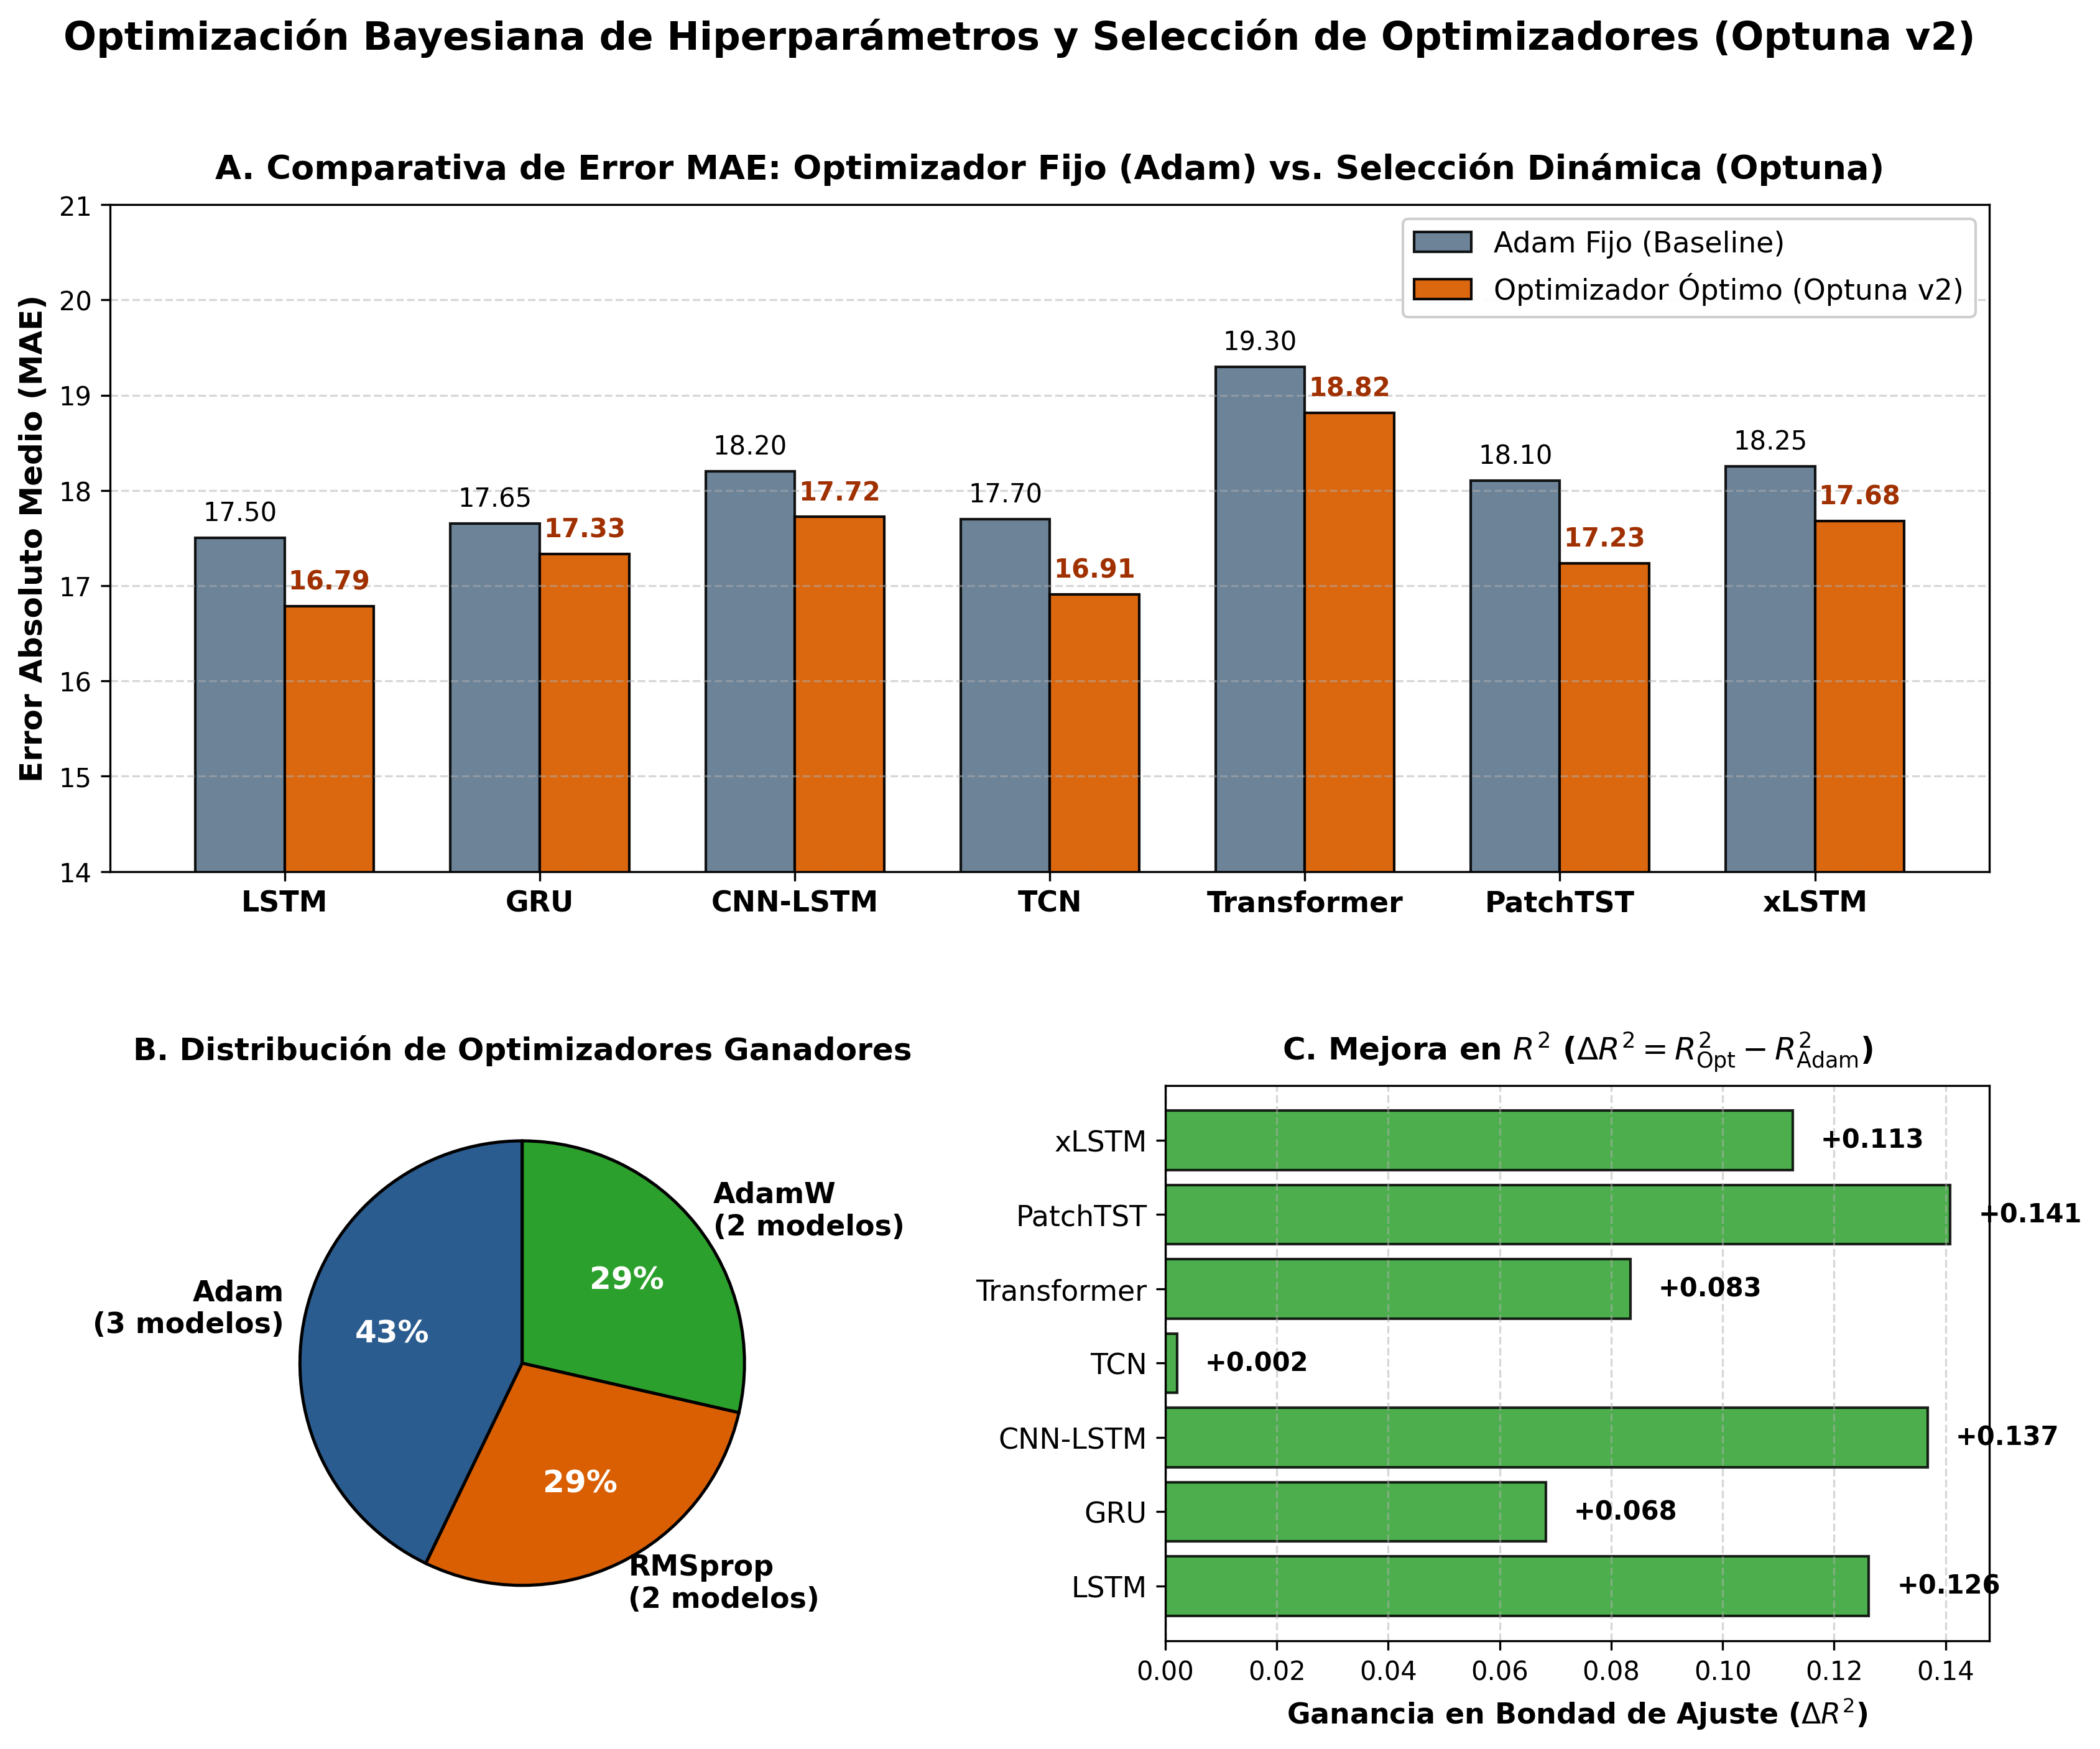
\includegraphics[width=0.86\textwidth]{figures/optuna_optimizadores_personalizados.png}
    \caption{Optimización bayesiana de hiperparámetros con Optuna v2: (A) comparativa de error MAE entre optimizador estándar (Adam) y selección dinámica guiada por TPE, (B) distribución de frecuencias de los optimizadores ganadores para cada arquitectura, y (C) ganancia neta en el coeficiente de determinación ($\Delta R^2$).}
    \label{fig:optuna_curves}
\end{figure}


% ======================================================================
\section{Validación Formal de las Hipótesis Científicas}
\label{sec:res_validacion_hipotesis}
% ======================================================================

\begin{itemize}
    \item \textbf{Validación de la Hipótesis~\ref{hip:h1} (\textsc{Aceptada}):} Las redes neuronales profundas superan de forma rotunda a los modelos clásicos en generalización inter-sujeto. Mientras que los modelos tabulares colapsan con $R^2 < -2.4$ en validación cruzada a ciegas, las arquitecturas recurrentes y convolucionales logran reducir el MAE medio a $\approx 17$ puntos VAS, demostrando su capacidad para extraer invariantes temporales de las bioseñales.
    \item \textbf{Validación de la Hipótesis~\ref{hip:h2} (\textsc{Aceptada Parcialmente}):} La arquitectura \xlstm{} (con celda \slstm{}) demuestra una notable estabilidad numérica y supera a la LSTM clásica en MAE global ($17.33$ frente a $17.50$) con menor número de parámetros (625k frente a 887k). No obstante, la GRU logra una ventaja marginal ($16.99$), situando a \xlstm{} como un competidor recurrente de primer nivel pero sin hegemonía absoluta en este dataset.
    \item \textbf{Validación de la Hipótesis~\ref{hip:h3} (\textsc{Aceptada}):} Los Modelos Fundacionales demuestran una capacidad notable de transferencia \textit{zero-shot} (Chronos logra el mejor MAE en fatiga física: $14.11$), pero requieren modelos de 710 millones de parámetros y backbones que multiplican por más de 1000 la memoria de un modelo recurrente ligero como GRU o \xlstm{}.
\end{itemize}


% ======================================================================
\section{Análisis de Limitaciones del Estudio}
\label{sec:res_limitaciones}
% ======================================================================

\begin{enumerate}
    \item \textbf{Tamaño de la Muestra ($N=12$ participantes):} Aunque cada sujeto aporta múltiples horas de registros multicanal a altas frecuencias, la cohorte de 12 individuos limita la diversidad fisiológica basal. Ampliar el dataset con mayor heterogeneidad etaria y clínica mejoraría la estabilidad de los estimadores de $R^2$.
    \item \textbf{Artefactos de Movimiento en Sensores de Muñeca (E4):} Durante tareas de alta intensidad física (carrera en cinta rodante), la señal óptica de fotopletismografía (BVP) en la muñeca sufre desacoplamientos mecánicos transitorios, requiriendo un mayor filtrado adaptativo.
    \item \textbf{Subjetividad Residual en las Etiquetas VAS:} Las escalas visuales analógicas presentan un sesgo de calibración intrínseco a cada persona (lo que un sujeto evalúa como fatiga 60 puede equivaler a un 80 para otro sujeto más autoexigente).
\end{enumerate}
